\chapter{Planning and resources evaluation}


\section{Planning}
This section presents de organisation of the project work. To facilitate its development process, the project was divided into a set of tasks, as outlined below. Trello~\cite{trello} was used to manage the development process, organise pending tasks and track progress throughout the project.

\begin{itemize}
    \item \textbf{Project analysis} (10 hours):
    \begin{itemize}
        \item \textbf{Meetings and research} (6 hours): In order to ensure that the game would adequately meet the educational needs and align with the objectives of the training activity, a number of meetings were held with the teachers involved, both during the initial phase and throughout the course of the project. These sessions made it possible to gather ongoing feedback and guide design and development decisions. The teachers also provided material about the garden, its species and the educational activities carried out there, which required additional research in order to understand the context and adapt the game content appropriately. Furthermore, to address certain technical aspects of the project, contact was maintained with a geolocation specialist, whose advice helped to resolve specific issues relating to this area.  
        \item \textbf{Initial planning} (4 hours): The initial planning phase consisted of defining the scope of the project, identifying the main tasks to be carried out and estimating the time required for each development stage.
    \end{itemize}

    \item \textbf{Game design} (50 hours): The game design phase is an ongoing process, as the project is constantly evolving. A key aspect of game design is ensuring that the focus of the serious game is not lost sight of. This includes ensuring the game is well-balanced, designing cooperative missions, and making sure the game is rewarding for the user, while meeting the pedagogical goals.
    
    \item \textbf{Art design} (10 hours): This task involved both sourcing and creating the visual and audio assets used in the game. Part of this time was spent searching for references and assets that matched the project’s artistic style and narrative, primarily through platforms such as the Unity Asset Store~\cite{unity_asset} and Itch.io game-assets~\cite{itch_io}. It also involved creating or adapting certain necessary resources, such as the character sprites, the images for the Garden of Hearing, and the image representing the mycorrhizae found above each garden. Furthermore, audio resources were explored for the Garden of Hearing quest, including testing recorded sounds and searching specialised sound databases such as Xeno-canto~\cite{xenocanto}, which offers recordings of birdsong and other natural sound material.
    
    \item \textbf{Development} (120 hours): This was the longest phase of the project and the one with the most iterations. It was divided into several implementation milestones, which are detailed below, including geolocation, multiplayer mode, mission logic and final integration.
    \begin{itemize}
        \item \textbf{Geolocation} (60 hours): Geolocation was the most complex part of the development process. This task required an initial research phase to understand the available location services and their limitations, followed by several rounds of implementation and testing. Its complexity was compounded by the difficulty of validating GPS behaviour outside the development environment, as reliable testing had to be carried out at the actual physical location.
        \item \textbf{Multiplayer} (20 hours): This task involved researching multiplayer functionality and subsequently implementing the system using the Unity Relay SDK. It included configuring the network service, creating and joining game sessions, as well as ensuring the necessary data synchronisation between players.
        \item \textbf{Quests} (30 hours): This task focused on designing, implementing and refining the quest system. Each quest had a different narrative and pedagogical purpose, which required specific mechanics, interaction models and feedback systems.
        \item \textbf{Integration} (10 hours): This task involved bringing together all the previously implemented elements and ensuring they functioned as a single, coherent prototype. Specifically, this involved integrating the geolocation system, the multiplayer functionality, the mission logic and user interaction, as well as testing the application’s entire workflow from start to finish in order to iterate and improve it.
    \end{itemize}

    \item \textbf{Testing and iteration} (60 hours): Aquí se ha contabilizado el tiempo de testear cada mecánica de las quest y el tiempo de ir a testear la geolocalización.
    
    \item \textbf{Documentation} (50 hours): This task covered the preparation of the project documentation throughout the development process.
    \begin{itemize}
        \item \textbf{The technical proposal} (5 hours): The technical proposal defined the scope of the project. Its aim was to set out the basic concept of the project, the educational context, the main objectives and the initial planning. This document also helped to clarify important conceptual aspects of the project, such as the distinction between gamification and serious games.
        \item \textbf{GDD} (10 hours): This document defined the core gameplay loop, cooperative mechanics, narrative framework, level structure, interface design, multiplayer model and technical architecture.
        \item \textbf{The Dissertation} (25 hours): The final report is a more comprehensive piece of documentation; for this reason, it was planned to include the theoretical underpinnings of serious games, the rationale behind the project, design decisions, and so on. The previous documents served as the basis for this report, but the content had to be reorganised and expanded from an academic perspective.
        \item \textbf{Project defence} (10 hours): Finally, the presentation was left until the final phase of the project, once all design and implementation decisions had been made. The presentation was a summary of the most relevant aspects of the project.
    \end{itemize}
\end{itemize}

Figure \ref{fig:gantt} presents the final Gantt chart of the project, including the tasks carried out and the time allocated to each of them.

\vspace{.5cm}
\begin{landscape}
\begin{figure}[htpb]
    \centering
    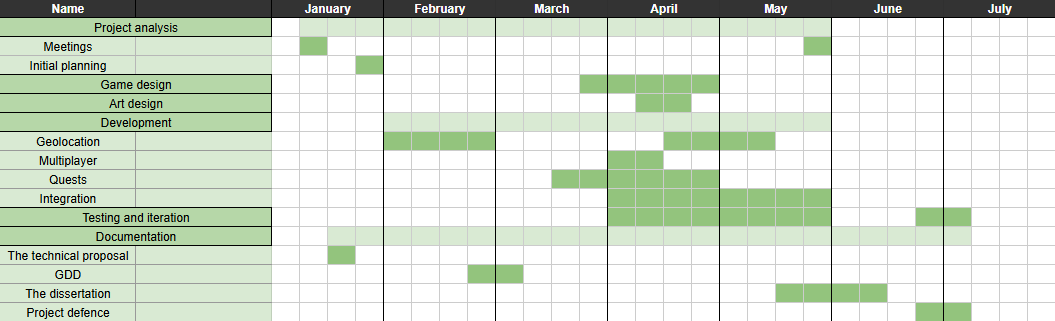
\includegraphics[width=\linewidth]{img/DiagramaGantt.png}
    \caption{Gantt chart of the project planning}
    \label{fig:gantt}
\end{figure}
\end{landscape}

\section{Costs}
The cost of carrying out this project is broken down below. This does not represent an actual payment, as the project was undertaken as an academic assignment, but it provides an estimate of the professional value of the work carried out

\subsection{Working hours}
The cost of the work carried out in this project has been estimated according to the number of development hours planned in the Gantt chart.  To assign an economic value to these hours, the reference used was the national collective agreement for consultancy and information technology companies, published in the Spanish Official State Gazette (BOE)~\cite{boe_convenio}.


The selected professional category was Area 3, Group D, Level 3, since it corresponds to software development and programming tasks and represents an appropriate reference for an entry-level profile in the software industry.
According to the updated 2026 salary tables, this category has an annual gross salary of 18,542.34 €. Considering the annual working time of 1,800 hours established in the same agreement, the hourly cost is calculated as follows:


\[
\frac{18{,}542.34\,\text{€}}{1{,}800} = 10.30\,\text{€/hour}
\]

Therefore, the estimated labour cost of the project is: 

\[
\text{Total labour cost} = \text{Number of hours} \times 10.30\,\text{€/hour}
\]

If the project required 330 hours of work: 

 \[
330\,\text{h} \times 10.30\,\text{€/h} = 3,399\,\text{€}
\]

\subsection{Hardware}
The development of a similar project would require a computer capable of running the necessary development tools primarily Unity as well as several mobile devices, between two and six devices. We will estimate six devices to be able to test the application under full conditions. The hardware specifications of the system used for this project is described below.
\begin{itemize}
    \item OMEN Gaming Laptop 16-ap0xxx~\cite{hp_omen}, 32GB of RAM and 954GB of hard disk, NVIDIA GeForce RTX 5070 Laptop GPU. Cost: 1,399€.
    \item Xiaomi Redmi Note 13 Pro 5G~\cite{redmi_note}. Cost: 80€
\end{itemize}

In order to provide a realistic cost reference to replicate the project, two alternative scenarios can be considered: purchasing a similar device or renting additional test devices.
The official Xiaomi reference price for the Redmi Note 13 Pro 5G is approximately 219.99 €. As another option, the company could rent one or two additional Android devices during the validation period. Although the exact Xiaomi Redmi Note 13 Pro 5G was not available in the consulted renting catalogue, similar Android devices were available through Rentik / Phone House~\cite{rentik}, such as the Xiaomi Redmi Note 15C from 6.90 €/month, the Motorola G55 5G from 8.90 €/month, or the Xiaomi Redmi Note 14 5G from 16.90 €/month.

The current range is between 6.90 €/month and 16.90 €/month, so an average cost of approximately 10 €/month/device will be estimated. Considering that, during one month, only two devices may be needed for testing, but during another month, up to six devices may be required.Therefore, the estimated cost would be 20 € for the first month plus 60 € for the second month, resulting in a total of approximately 80 €.


\subsection{Software}
The software tools and licences required to develop this project were free for educational use, but their commercial value is detailed below for replication in a professional setting:
\begin{itemize}
    \item \textbf{Unity:} Used as the main game engine. While it currently offers a free Personal edition, the pricing structure was recently modified, cancelling the Runtime Fee~\cite{unity_pricing}. For a professional studio, a Unity Pro licence might be required depending on revenue.
    \item \textbf{ArcGIS SDK:} Used for the map and geolocation features. A student use licence~\cite{arcgis_license} is available at no cost for academic purposes, whereas commercial development requires a paid subscription.
    \item \textbf{OpenAI Codex:} Used to assist in the development of certain scripts and technical problem-solving. The pricing model~\cite{codex_pricing} is 20 US\$/month/user. The 300 hours of project development took around 4 months, so this would cost around 4 × 20 = 80 €.
\end{itemize}
\subsection{Other expenses}
Since the project is based on a geolocated experience in the \textit{Jardín de los Sentidos}, several field tests had to be carried out in the real environment to validate GPS behaviour, interaction areas and mobile usability. Therefore, travel expenses were included as an additional project cost.
Each validation trip was estimated as a 15 km journey. Using the official Spanish reference of 0.26 €/km for private vehicle travel expenses, the cost per visit is:
Number of visits × 15 × 0.26 = Travel cost      
15 × 0.26 = 3.9€/visit
Assuming a total of  ten validation visits, the estimated travel cost would be:
10 × 3.9 =  39€

\subsection{Estimated total cost}
After analysing the different cost categories, the estimated cost of replicating the project in a professional context amounts to 4,798 €. This total includes the estimated labour cost, the hardware required for development and testing, the software tools and licences, and the travel expenses associated with field validation. Table ~\ref{tab:general_costs} summarises the final cost breakdown for each category.




\vspace{1cm}
% Tabla general de costes
\begin{table}[htpb]
\centering
\caption{General project cost, broken down into the main cost categories}
\label{tab:general_costs}
\renewcommand{\arraystretch}{1.5}
\begin{tabular}{>{\raggedright\arraybackslash}p{0.5\textwidth} >{\raggedleft\arraybackslash}p{0.3\textwidth}}
\rowcolor[HTML]{B0C9B0} \textbf{Concept} & \textbf{Cost (€)} \\
\rowcolor[HTML]{F0F5F0} Working hours & 3,399 €\\
\rowcolor[HTML]{DFE8DF} Hardware & 1,479 €\\
\rowcolor[HTML]{F0F5F0} Software & 80 €\\
\rowcolor[HTML]{DFE8DF} Other expenses & 39 €\\
\hline
\rowcolor[HTML]{B0C9B0} \textbf{Total} & \textbf{4,997 €} \\
\end{tabular}
\end{table}

\section{Planning Deviations}

\begin{table}[htpb]
\centering
\caption{Planning deviations}
\label{tab:planning_deviations}
\renewcommand{\arraystretch}{1.5}
\begin{tabular}{
>{\raggedright\arraybackslash}p{0.35\textwidth}
>{\raggedleft\arraybackslash}p{0.22\textwidth}
>{\raggedleft\arraybackslash}p{0.20\textwidth}
>{\raggedleft\arraybackslash}p{0.14\textwidth}
}
\rowcolor[HTML]{B0C9B0} 
\textbf{Task} & \textbf{Estimated hours} & \textbf{Hours worked} & \textbf{Deviation} \\

\rowcolor[HTML]{F0F5F0} Project analysis & 15 & 10 & -5 \\
\rowcolor[HTML]{DFE8DF} Game design & 80 & 50 & -30 \\
\rowcolor[HTML]{F0F5F0} Art design & 15 & 10 & -5 \\
\rowcolor[HTML]{DFE8DF} Development & 130 & 150 & +20 \\
\rowcolor[HTML]{F0F5F0} Testing and iteration & 30 & 60 & +30 \\
\rowcolor[HTML]{DFE8DF} Documentation & 30 & 50 & +20 \\
\hline
\rowcolor[HTML]{B0C9B0} 
\textbf{Total} & \textbf{300} & \textbf{330} & \textbf{+30} \\
\end{tabular}
\end{table}


The project presented several deviations from the initial planning. As shown in Table~\ref{tab:planning_deviations}, the final workload exceeded the initial estimation by 30 hours. Table~\ref{tab:planning_deviations} shows the comparison between the initially estimated hours, the hours finally spent on each task, and the resulting deviation.

The tasks that required less time were project analysis, game design and art design. In the case of project analysis, the scope of the project and the main requirements were defined at an early stage, mainly thanks to the initial meetings with the teachers involved in the educational activity. Game design also required fewer hours than initially planned because some design decisions were simplified during development in order to keep the prototype feasible and focused on the main educational objectives. Similarly, art design took less time than expected because several visual resources were obtained from existing asset libraries or adapted from available material, reducing the need to create every asset from scratch.

In contrast, development, testing and documentation required more time than originally estimated. Development exceeded the initial planning because the implementation of geolocation and the integration of the different systems involved more technical complexity than expected. The project required several iterations to connect the map, GPS position and mission flow, since the application could not be validated inside the Unity editor. The geolocation system had to be tested on Android devices and in the real physical environment of the \textit{Jardín de los Sentidos}.

The project was completed in 330 hours instead of the 300 hours initially estimated. The final deviation of 30 hours was mainly caused by the complexity of developing and validating a geolocated mobile application in a real outdoor environment.